\chapter{Grundlagen}
In diesem Kapitel wird das Grobkonzept von Skatemate dargestellt, um einen Überblick über das Elektroskateboard zu geben. Bevor im Kapitel 3 die dazu notwendigen Grundlagen erklärt werden, wird die Bedienung von Skatemade erklärt, so dass die Grundlagen besser eingeordnet werden können. 
\section{Grobkonzept}
Skatemate kann in drei Grundbereiche unterteilt werden: Die Steuerung über den Magic-Glove, die Motoransteuerung mittels FOC und die Stromversorgung mitsamt dem selbst konzipierten Akkuladegerät. Wie diese drei Bereiche miteinander interagieren ist im Blockschema \ref{fig:grobkonzeptblockschaltbildgrob}  dargestellt. Die Antriebstechnik ist über ein Kabel mit der Stromversorgung verbunden, die Inputs der Steuerung erhält sie über ein Funknetz. Nachfolgend werden die drei Bereiche detaillierter erläutert. Zudem wird darauf eingegangen, weshalb diese Lösung gewählt wurde. 
\begin{figure}[H]
	\centering
	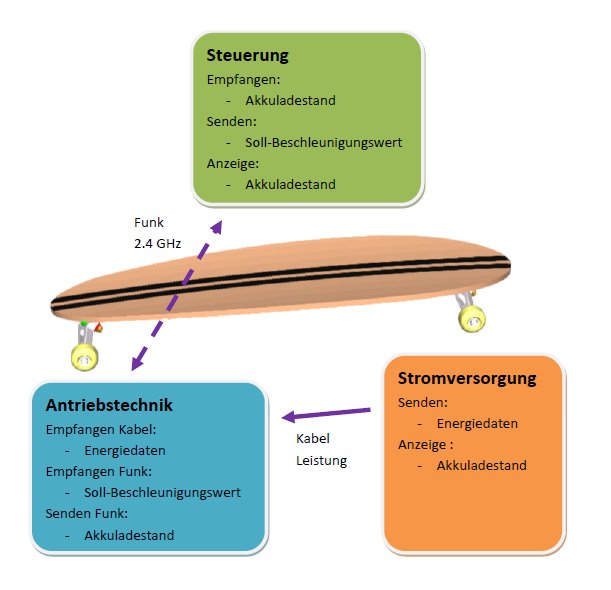
\includegraphics[width=0.7\linewidth, keepaspectratio]{images/Grobkonzept_Blockschaltbild_grob}
	\caption[Blockschaltbild Grobkonzept]{Blockschaltbild Grobkonzept}
	\label{fig:grobkonzeptblockschaltbildgrob}
\end{figure}

\subsection*{Steuerung über den Magic-Glove}
Es gibt verschiedene Wege, wie ein Elektrisches Skateboard gesteuert werden kann. Eine Variante ist, über Drucksensoren im Brett durch eine Gewichtsverlagerung in Fahrtrichtung eine Geschwindigkeitsregulation zu erreichen. Da auf unebenem Gelände eine natürliche Gewichtsverlagerung entsteht, und diese kompensiert werden müsste, und zudem lokal beschränkte Sensoren die Bewegungsfreiheit auf dem Skateboard einschränken können, wurde diese Variante verworfen. Stattdessen wird die Geschwindigkeit über eine Fingerbewegung gesteuert. Dazu wird ein Handschuh mit integrierten Sensoren entwickelt. Dieses Wearable enthält einen Flex Sensor, der die Beugung des Zeigefinders misst. Diese Beugung wird Quantifiziert und als Sollbeschleunigung der Motoransteuerung übergeben. Dies geschieht über ein 2.4 GHz Funknetz, dazu ist ein Funkmodul integriert. Die Stromversorgung erfolgt über eine XXXY Batterie. 

\subsection*{Antriebstechnik}
Als Antrieb ist der OX1 2-10 Motor vorgegeben, dies ist ein Brushless-Gleichstrommotor (BLDC-Motor). Er verfügt nicht über Hallsensoren. Die technischen Hintergründe des Motors werden im Kapitel xxx gegeben. Ein BLDC-Motor ist wie ein permanentmagnetischer Drehstrom-Synchronmotor (PMSM) aufgebaut. 
Die Ansteuerung kann über eine Kommutierung oder eine Vektorregelung erfolgen\cite{BLDC} [ Quelle xxx ]. Die Kommutierung kann prinzipiell gesteuert oder ungesteuert erfolgen. Bei der ungesteuerten Kommutierung kann der Motor als Schrittmotor genutzt werden, die Rotorposition folgt der Steuerung. Diese Variante ist für ein gleichmässig rollendes Skateboard ungeeignet. Die Kommutierung muss also abhängig von der Rotorposition erfolgen (geführte Kommutierung), die Steuerung reagiert also auf die effektive Rotorposition und passt sich dieser an (xxx)  Am einfachsten wäre diese mit Sensoren, da unser Motor jedoch nicht über Sensoren verfügt, muss der Motor über eine sensorlose gesteuerte Kommutierung angesteuert werden. Dies funktioniert jedoch nur ab einer Mindestdrehzahl wirklich gut. Zum Anfahren muss der Motor speziell angesteuert werden. 
Bei der Vektorreglung, in diesem Fall eine Feldorientierte Regelung (field oriented controll, FOC), werden die Spannungen zur Steuerung aktiv der Rotorlage angepasst. Auch mit der FOC kann zwischen sensorgesteuerte und sensorlosen Regelung unterschieden werden. Bei der sensorlosen Regelung muss wiederum zum Anfahren eine zusätzliche Ansteuerung erfolgen. Diese wird im Kapitel xxx erklärt. Kann die Anfangsposition jedoch genügen genau geschätzt werden, läuft der Motor auch bei tiefen Geschwindigkeiten gleichmässig, da er relativ genau geregelt werden kann. Dies entspricht unseren Anforderungen für das Skatemate, da ein sanftes Anfahren sehr wichtig ist. Die FOC ist im Kapitel  xxx erklärt .

\subsection*{Stromversorgung}


-------------------------------------------------
NOCH NICHT EINGEBUNDEN! 

\begin{figure}[H]
	\centering
	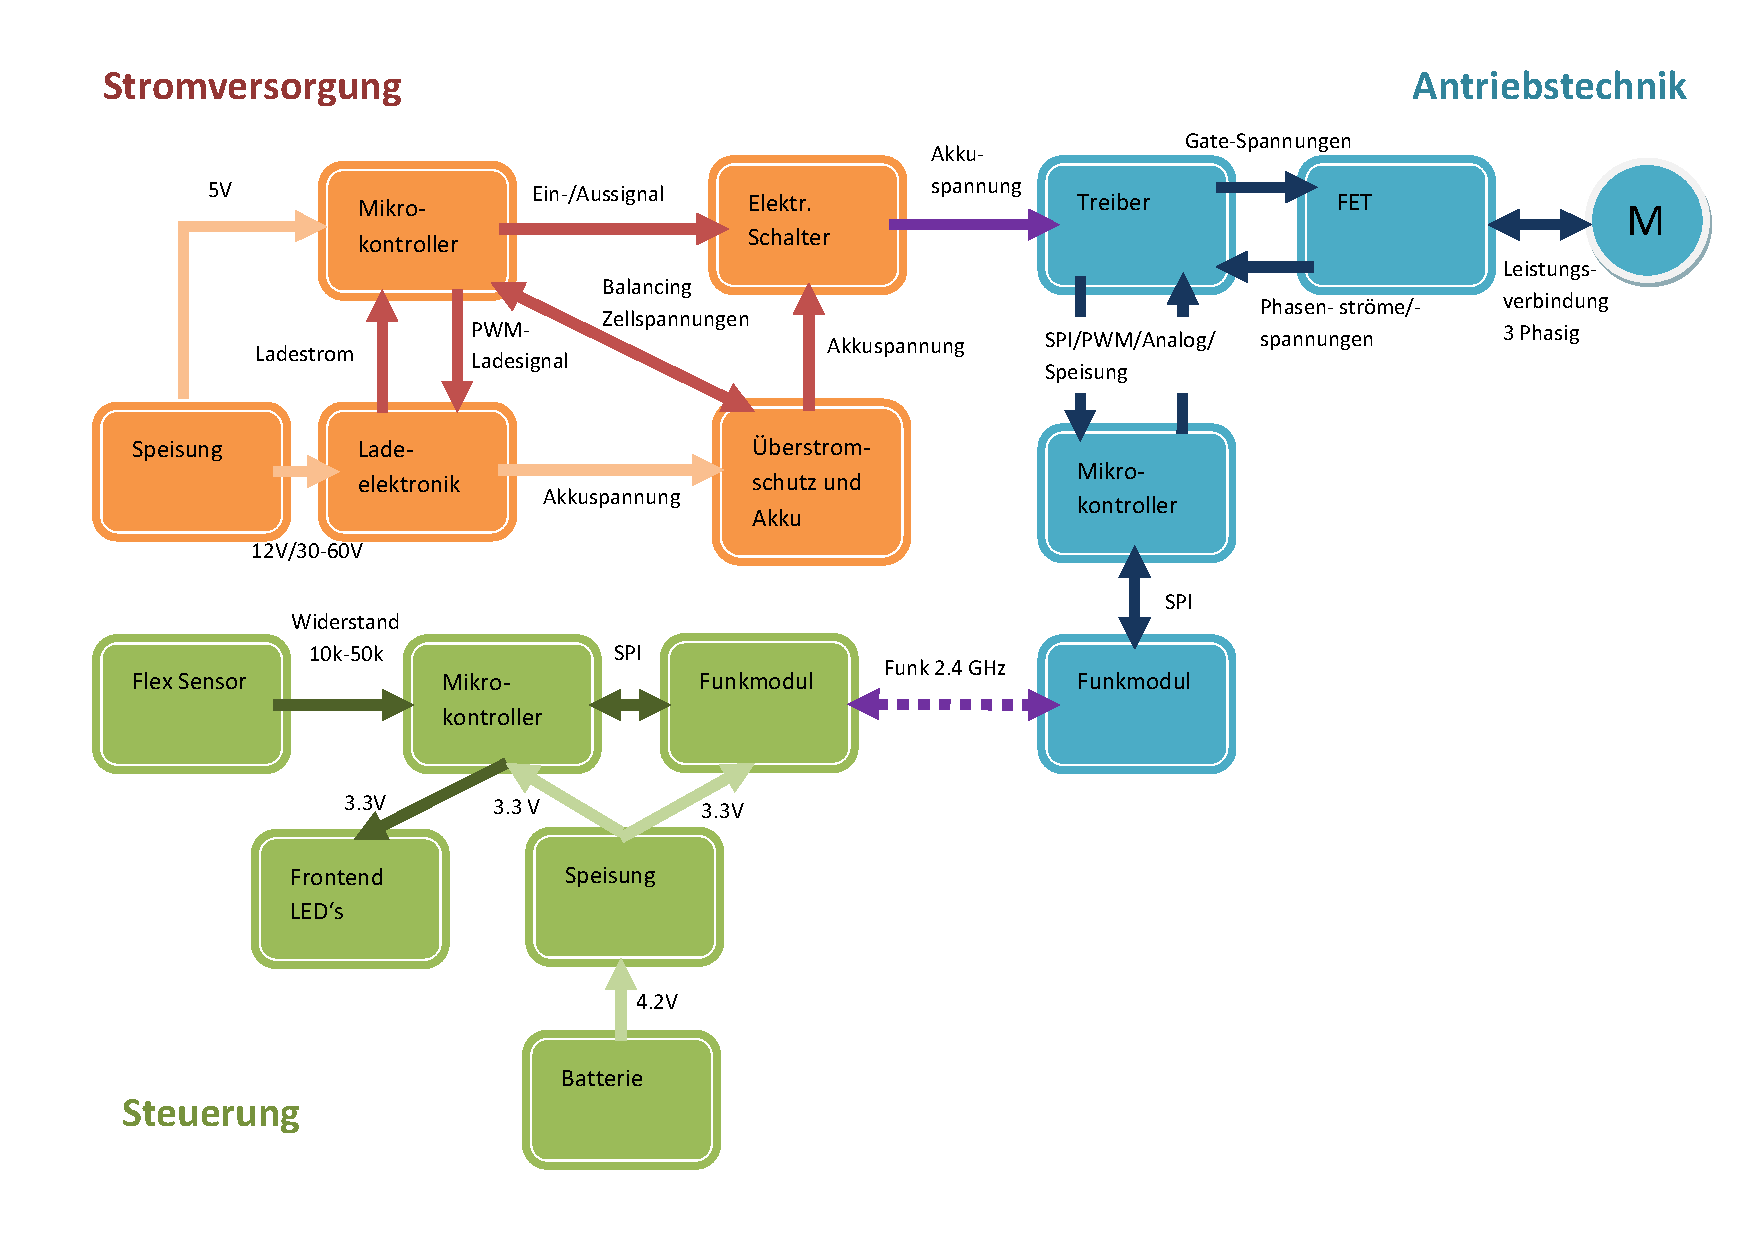
\includegraphics[width=\linewidth]{images/Grobkonzept_Blockschaltbild_detailliert}
	\caption[Detailliertes Blockschaltbild]{Detailliertes Blockschaltbild}
	\label{fig:grobkonzeptblockschaltbilddetailliert}
\end{figure}



%\begin{figure}[H]
%	\begin{center}
%		\includegraphics[width=\textwidth, height=50mm, keepaspectratio]{ekg_grundlagen}
%		\caption{Das Herz als Dipol \cite{Herz_als_Dipol}}
%		\label{ekg_grundlagen}
%	\end{center}		
%\end{figure}

\section{Bedienung}
